%% Digital Systems
%% Introduction
\def\FileDate{98/11/04}
\def\FileVersion{1.0}
% ----------------------------------------------------------------
% Notes pages *********************************************************
% ----------------------------------------------------------------

\begin{slide}\label{slide:l7s1}
\heading{Introduction}
\begin{itemize}
\item Digital systems are important in modern technology because they
  are used extensively to implement designs that previously used
  analogue (continuous) technology.
\item The concepts developed for continuous systems
  are all applicable to digital systems.
\item This introduction commences with digital signals, continues with
  digital systems, and ends with an overview of how analogue systems
  may be converted to digital systems.
\end{itemize}
\end{slide}

\begin{slide}\label{slide:l7s1a}
\heading{Analogue v Digital}
\begin{itemize}
\item The real world we inhabit is analogue. We process analogue
  signals: e.g. vision and sound. Physical systems are analogue
  systems of force, velocity, current, voltage, temperature pressure,
  etc.
\item Advances in electronics means that more and more of the storage,
  distribution and processing of signals is actually done using
  digital technology.
\item There have to be methods of converting analogue to digital (e.g.
  recording of sound) and digital to analogue (e.g. signals delivered
  by loudspeakers).
\item We need to be able to model the signals, their conversion and
  the systems that process them.
\end{itemize}
\end{slide}

\section*{Samplers and Discrete-Time Physical Systems}

As hinted in the introduction, we need to convert analogue signals to
digital signals before the digital signal can be stored, distributed and
manipulated by a digital system. At the point of delivery, we need to
convert the signal back into digital form. In this section we
introduce the signal conversion devices and give an example of one
commonly seen digital system.

\subsection*{Analogue to Digital Converter}

We begin by describing the \emph{digital to analogue converter} (D/A
or DAC), since this device is usually also a component of the
\emph{analogue to digital compensator} (A/D or ADC). We assume that
the DAC receives a digital signal, in the form of a binary number,
every $T$ seconds (usually from a digital computer, micro-controller or
a digital signal processor). The DAC converts the binary number to a
constant voltage equal to the value of that number, and outputs this
voltage until the next number arrives and the DAC input. The block
diagram of the DAC and a typical response is shown in
\sref{slide:DAC}.

\begin{slide}\label{slide:DAC}
\heading{Digital to Analogue Converter (D/A or DAC)}
\begin{center}
  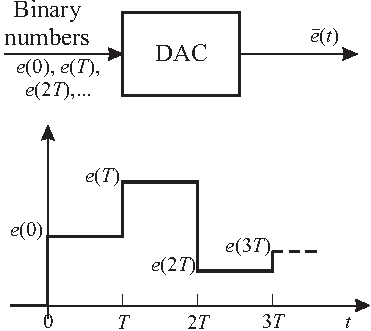
\includegraphics{pictures/DAC.pdf}
\end{center}
\end{slide}

We next describe a comparator, which is also a component of the ADC. A
comparator and its characteristics are illustrated in
\sref{slide:compare}. The input voltage $v_i(t)$ is compared with the
reference voltage $v_r(t)$.  If $v_i(t) > v_r(t)$ the comparator
outputs logic ``1''; for example logic 1 is 5V for TTL logic.  If
$v_i(t) < v_r(t)$ the comparator outputs logic ``0''; which is less
than 1V for TTL logic. The signal ground is normally omitted from
circuit diagrams, but all voltages are compared relative to signal
ground.

\begin{slide}\label{slide:compare}
\heading{Voltage Comparator}
\begin{center}
  \resizebox{250pt}{!}{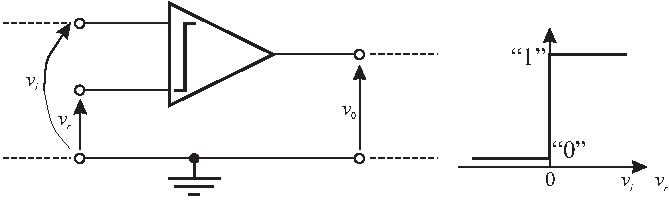
\includegraphics{pictures/comparator.pdf}}
\end{center}
\end{slide}

Several circuits are used to implement an analogue to digital
converter. Each circuit has different characteristics. We illustrate
the up-counter ADC shown in \sref{slide:ADC}. The $n$-bit counter is
reset to zero when the start-of-conversion (SOC) signal is received by
the device. The count increases by 1 with the arrival of each clock
pulse. The $n$-bit DAC converts the binary equivalent of the count to
a voltage $v_R$. 

\begin{slide}\label{slide:ADC}
\heading{Analogue to Digital Converter}
The counter ADC.
\begin{center}
  \resizebox{300pt}{!}{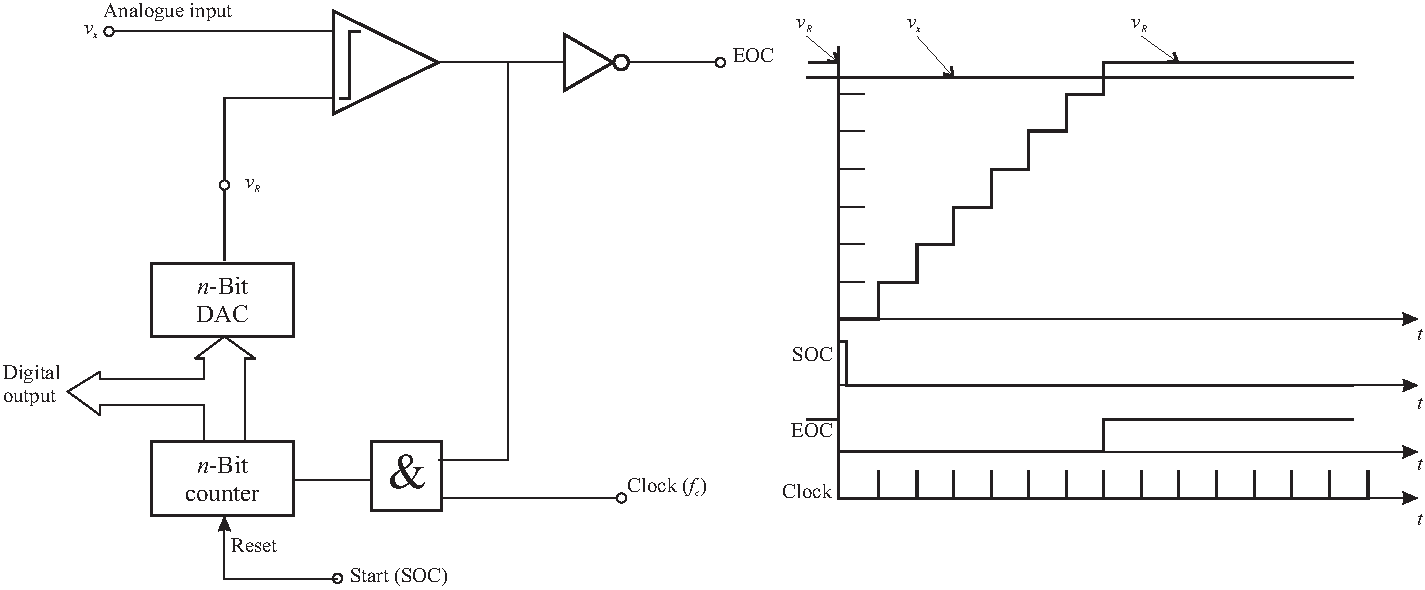
\includegraphics{pictures/ADC.pdf}}
\end{center}
\end{slide}

The analogue voltage $v_x$ to be converted is compared to $V_R$. When
$V_R$ becomes greater than $v_x$, the comparator outputs a logic 0,
which halts the clock input through the AND gate. The
end-of-conversion (EOC) pulse then signals that the digital equivalent
to $v_x$ is ready. The counter output can then be read from the
digital output as a binary number which is approximately equal to the
analogue input.

\subsection*{Digital Systems}

Once we have the ability to convert analogue signals into binary
numbers and back, we have the ability to process the information using
computers and other digital devices. A familiar device will be the
compact disk (CD) player.

\begin{slide}\label{slide:CD1}
\heading{Compact Disk (Analogue to Digital)}
\begin{itemize}
\item Continuous time signal is filtered with an ``anti-aliasing''
  band-pass filter with bandwidth of 5 to 20,000 Hz.
\item Filtered audio signal sampled using ADC at 44,100 samples per second and
  with 14-16 bits precision. 
\item Each sample is stored, along with error
  correcting bits, as a stream of binary codes. 
\item The codes are recorded using microscopic pits etched into the surface of the CD.
\end{itemize}
\end{slide}

\begin{slide}\label{slide:CD2}
\heading{Compact Disk (Digital to Analogue)}
\begin{itemize}
\item For stereo music, two channels are sampled and stored.
\item Data is stored on a continuous track that spirals outwards from
  the centre.
\item Data is read at a constant rate (44,100 Hz) and is processed (e.g.
  error corrected and buffered for tilt control) before being
  converted, using DAC, to a signal that can be delivered to a
  loudspeaker.
\item Velocity of disk needs to be controlled so that it decreases as
  the radius of the track increases. Position and the focus of the laser used to read the data is
  also controlled.
\item Audio CD holds approx. 540 MBytes of data which is enough to
  store 74 minutes of stereo music.
\end{itemize}
\end{slide}


\section*{Generation of Digital Signals}
Digital signals do not occur naturally. They are generated by
sampling continuous signals, or by digitally processing other
digital signals. Sampling is accomplished by a sampler known as an
``\emph{Analogue to Digital Converter (ADC)}''.

\begin{slide}\label{slide:l7s2a}
  \heading{Sampling and Sequences}
  \begin{itemize}
   \item Sampling -- mathematical model of the ADC
   \item Sampled signals are modelled as sequences
   \item Sequences can be shifted backwards and forwards
   \item The advance and delay operators are analogies to the derivative
     and integral operators
  \end{itemize}
\end{slide}

\begin{slide}\label{slide:l7s2}
  \heading{Sampling -- Mathematical model of the ADC}
  \center{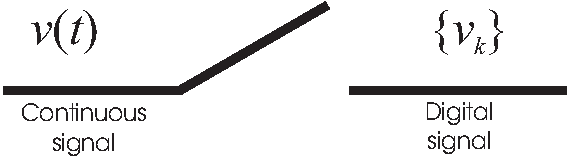
\includegraphics{pictures/sampler.pdf}}
  \begin{itemize}
   \item Quantisation, introduced by converting an analogue signal to a
     binary number with a finite number of bits, will not be considered. 
  \end{itemize}
\end{slide}


The analogue to digital converter is modelled as a a switch as
shown in \sref{slide:l7s2}. 

\ifslidesonly
\begin{slide}
\heading{Modelling Sampling: Sequences}
% chunk 1
The equivalent of the differential equation model for continuous
systems is the difference equation for digital systems.

Replacing
the differential operator $\frac{d}{dt}$ by the advance operator
$\triangle$ gives the general form of the difference equation as
\begin{equation}\label{eq:l9e1}
  \triangle^ny + a_{1}\triangle^{n-1}y + \ldots +  a_n y = b_0
  \triangle^n u + b_{1}\triangle^{n-1} u + \ldots + b_n u.
\end{equation}

\endinput

\end{slide}
\fi
% chunk 1
The equivalent of the differential equation model for continuous
systems is the difference equation for digital systems.

Replacing
the differential operator $\frac{d}{dt}$ by the advance operator
$\triangle$ gives the general form of the difference equation as
\begin{equation}\label{eq:l9e1}
  \triangle^ny + a_{1}\triangle^{n-1}y + \ldots +  a_n y = b_0
  \triangle^n u + b_{1}\triangle^{n-1} u + \ldots + b_n u.
\end{equation}

\endinput


\ifslidesonly
\begin{slide}
\heading{Modelling Sampling: Regular Sampling}
Only regular sampling will be considered. A constant period $T$~s
between sampling instants is equivalent to a sampling frequency
$\omega_s$~rad~s$^{-1}$, where \[ T = \frac{2\pi}{\omega_s}. \]

Sampling is assumed to be synchronized to the time origin $t=0$ so
that \[ v_k = v(kT)\ \mathrm{for\ all }\ k.\]
\endinput

%%% Local Variables: 
%%% mode: latex
%%% TeX-master: "notes"
%%% End: 

\end{slide}
\fi
Only regular sampling will be considered. A constant period $T$~s
between sampling instants is equivalent to a sampling frequency
$\omega_s$~rad~s$^{-1}$, where \[ T = \frac{2\pi}{\omega_s}. \]

Sampling is assumed to be synchronized to the time origin $t=0$ so
that \[ v_k = v(kT)\ \mathrm{for\ all }\ k.\]
\endinput

%%% Local Variables: 
%%% mode: latex
%%% TeX-master: "notes"
%%% End: 


\begin{slide}\label{slide:l7s3}
\heading{Sampling: The Signals}
\center{\resizebox{250pt}{!}{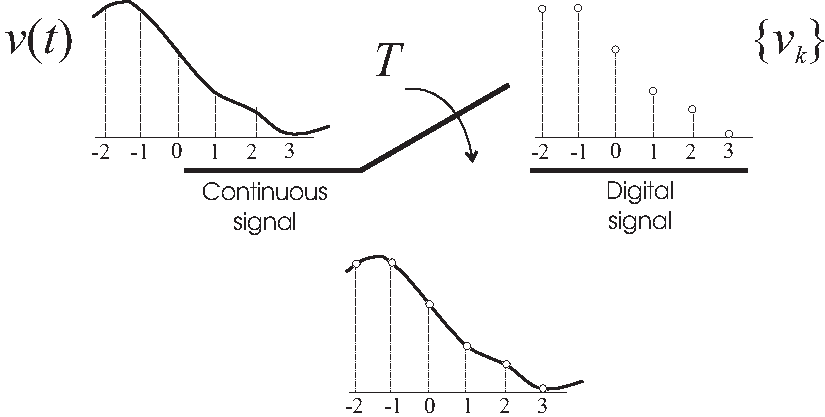
\includegraphics{pictures/sampling.pdf}}}
\end{slide}

\ifslidesonly
\begin{slide}
\heading{Indexing the Sequence}
The index $k$ denotes the current value. Digital signals will be
taken as zero prior to the time origin, in the same way as
continuous signals:
\[ v_k = v(kT) = 0\ \mathrm{for}\ k<0. \]

Except in cases where it is necessary to distinguish between them,
both the continuous signal $v(t)$ and the digital signal
$\left\{v_k\right\}$ will be denoted by $v$.
\endinput

%%% Local Variables: 
%%% mode: plain-tex
%%% TeX-master: "notes"
%%% End: 

\end{slide}
\fi
The index $k$ denotes the current value. Digital signals will be
taken as zero prior to the time origin, in the same way as
continuous signals:
\[ v_k = v(kT) = 0\ \mathrm{for}\ k<0. \]

Except in cases where it is necessary to distinguish between them,
both the continuous signal $v(t)$ and the digital signal
$\left\{v_k\right\}$ will be denoted by $v$.
\endinput

%%% Local Variables: 
%%% mode: plain-tex
%%% TeX-master: "notes"
%%% End: 


\section*{Shifting Digital Signals}
Shifting digital signals is the mechanism by which dynamic
behaviour is introduced into digital systems. The shifting
operators are comparable to differentiating and integrating
continuous signals.

\begin{slide}
  \heading{Forward Shifting a Digital Signal}\label{slide:l7s4}
\begin{itemize}

\item   The first forward shift of a digital signal $v$ is generated by
  applying the ``\emph{Advance Operator}'' $\triangle$  to give the
  advanced digital signal $\triangle v$, where \[ \triangle v = \triangle
  \{v_k\} = \{\triangle v_k\} = \{v_{k+1}\}.\]
  

\item   The signal $v$ is advanced by one value (a time advance of
  $T$). $v_0$ vanishes because $\triangle v$ is zero prior to $t=0$.


\item   Repeated operation gives the $r$-th forward shift \[
  \triangle^r v = \{v_{k+r}\}\].

\end{itemize}

\end{slide}

\begin{slide}
\heading{Advance and Derivative Operator}\label{slide:l7s4a}

\begin{itemize}

\item the advance operator $\triangle$ is equivalent to the derivative operator
  $d/dt$.

\item   Neither the advance operator $\triangle$ nor the derivative
  $d/dt$ is physically realistic. 

\item $\triangle$ is not realistic because
  the current value of $\triangle v$, which is $\triangle v_k$,
  is the \emph{future} value of $v_{k+1}$ of the signal $v$. 

\end{itemize}
\end{slide}

The Advance operator $\triangle$ for digital signals is equivalent to the
differential operator $d/dt$ for continuous signals. The first forward
shift $\triangle v$ $\equiv$ first derivative $dv/dt$. The $r$-th
forward shift $\triangle^r$ $\equiv$ $r$-th derivative $d^rv/dt^r$. Neither the $\triangle$ operator nor the $d/dt$ operator are
physically realistic.

\begin{slide}
  \heading{Backward Shifting a Digital Signal}\label{slide:l7s5}
\begin{itemize}

\item   The first backward shift of a digital signal $v$ is generated by
  applying the ``\emph{Delay Operator}'' $\nabla$  to give the
  delayed  digital signal $\nabla v$, where \[ \nabla v = \nabla
  \{v_k\} = \{\nabla v_k\} = \{v_{k-1}\}.\]
  

\item   The signal $v$ is delayed by one value (a time delay of
  $T$).


\item   Repeated operation gives the $r$-th backward shift \[ \nabla^r v = \{v_{k-r}\}.\]

\item the delay operator $\nabla$ is equivalent to the integral operator
  $\int$.

\item   The delay operator $\nabla$ is not only physically realistic
  but can be implemented easily by storage and retrieval in a digital
  computer.

\end{itemize}
\end{slide}

The delay operator $\nabla$ for digital signals is equivalent to the
integral operator $\int dt$ for continuous signals. The first backward
shift $\nabla v$ $\equiv$ first integral $\int v dt$. The $r$-th
backward shift $\nabla^r$ $\equiv$ $r$-th integral $\int \int \cdots
\int v dt$. Both the $\nabla$ operator and the $d/dt$ operator are
physically realistic.

\begin{slide}
  \heading{Mathematical and Computer Models}\label{slide:l7s6}
  \begin{itemize}
  \item Advance operators (like differential operators) are best suited
    to mathematical models.
  \item Delay operators (like integral models) are best suited to
    computer models.
  \end{itemize}
  In a \emph{Digital Operational Block Diagram} the fundamental
  dynamic operation is denoted by
  \begin{center}\resizebox{200pt}{!}{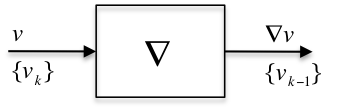
\includegraphics{pictures/blockd.png}}\end{center}
\end{slide}


%%----------------------------------------------------------------
%% The z transform
%%----------------------------------------------------------------

\begin{slide}\label{slide:l8s1}
\heading{Definition of the $z$ Transformation} 
\begin{itemize}
 \item The $z$ transformation has the same role in digital systems
 that the Laplace transform has in continuous systems.
 \item $z$ transformation of a digital signal $v$ is defined as \[V =
 V(z) = \mathcal{Z} v = \mathcal{Z} \{ v_{k} \}=\sum_{k=0}^{\infty}
 v_k z^{-k}.\] 

 \item Similarly, $v$ is the \emph{inverse $z$
 transform} of $V$, or
   \[\mathcal{Z}^{-1} V.\]

\end{itemize}

\end{slide}


\begin{slide}\label{slide:l8s1a}
\heading{$z$ Transform is a Summed Series (1)} 

\begin{itemize}

\item Obtaining $z$ transforms involves summing series. Often this is a
\emph{binomial} series \[(1+x)^r = 1 + rx + \frac{r(r-1)}{2}x^2 +
\cdots + \frac{r(r-1)\cdots(r-n+1)}{n!}x^n + \cdots\]

\item The transform pairs for common functions
are put into tables so that it is not necessary to sum a series in
most cases.

\end{itemize}

\end{slide}

\begin{slide}\label{slide:l8s1a1}
\heading{Example 1: $z$ Transform of The Unit Step} 

\begin{itemize}

\item If $v$ is the digital sequence $\{\epsilon_k\}$, that is
\[1\ 1\ 1\ 1\ 1\ \ldots\]

\item $z$ transform is
\[\sum_{k=0}^{\infty} 1\times z^{-k} 1x= 1 + z^{-1} + z^{-2}+\cdots\] 

\item this is summed
as a binomial series as \[(1-z^{-1})^{-1} = \frac{1}{1-z^{-1}} =
\frac{z}{z-1}.\] 

\end{itemize}
\end{slide}

\begin{slide}\label{slide:l8s1b}
\heading{Example 2: $z$ Transform of a Power Series} 

\begin{itemize}

\item Another example which is commonly found is the digital signal $v$
given by $\{v_k\} = \{\alpha^k\}$. 

\item The $z$ transform is
\[\sum_{k=0}^{\infty} \alpha^{k} z^{-k} = 1 + \alpha z^{-1} + \alpha^2
z^{-2}+\cdots\] 

\item $\ldots$ which is summed as a binomial series as
\[(1-\alpha z^{-1})^{-1} = \frac{1}{1-\alpha
  z^{-1}} = \frac{z}{z-\alpha}.\]

\end{itemize}

\end{slide}

\begin{slide}\label{slide:l8s1c}
\heading{Example 3: $z$ Transform of a Continuous Signal} 

\begin{itemize}

\item If the digital signal $v$ is generated by sampling the continuous
signal $v(t)$, then the transform $V$ also has a correspondence
with $v(t)$. 

\item For example, if \[v(t) = e^{-at}\] then \[v_k = v(kT)
= e^{-akT} = (e^{-aT})^k.\] 

\item $\ldots$ So, from the previous result, with
$\alpha=e^{-aT}$, we have the $z$ transform as
\[\frac{1}{1-e^{-aT}z^{-1}}=\frac{z}{z-e^{-aT}}.\]

\end{itemize}

\end{slide}

\section*{$z$ Transforms of the Shift Operators}

\begin{slide}\label{slide:l8s2}
\heading{\emph{z} Transform for Forward Shift}

\begin{itemize}
\item  This is similar to the derivative property of the Laplace
  transform.
 \[\mathcal{Z}\triangle v = z V(z) - zv_0\] It also introduces the initial member $v_0$.

\item  We can also show that
  \[\mathcal{Z}\triangle^2 v = z^2 V(z) - z^2 v_0 - z v_1\]
\item and in general
  \[\mathcal{Z}\triangle^r v = z^r V(z) - \sum_{i=0}^{r-1} v_i z^{r-i}.\]

\end{itemize}

\end{slide}

To prove the relationship illustrated in \sref{slide:l8s2} we note
that
\[\triangle v = v_1\ v_2\ v_3\ \ldots\ v_{k+1}\ldots\]
so that
\begin{eqnarray*}
  \mathcal{Z}\triangle v & = & v_1 z^0 + v_2 z^{-1} + v_3 z^{-3} + \cdots
  + v_{k+1}z^{-k}+\cdots \\
& = & z(v_0 + v_1 z^{-1} + v_2 z^{-2} + \cdots
  + v_{k+1}z^-{k+1}+\cdots)-zv_0\\
&=& zV(z) - zv_0.
\end{eqnarray*}
Similar arguments may be used to prove the other relationships
shown in \sref{slide:l8s2}.

\begin{slide}\label{slide:l8s3}
 \heading{$z$ Transform for Backward Shift}
\begin{itemize}
\item  This is similar to the integral property of the Laplace
   transform.
  \[\mathcal{Z}\nabla v = z^{-1} V(z)\]
\end{itemize}

\end{slide}

\section*{The Inverse z Transformation}
\begin{slide}\label{slide:l8s4}
   \heading{Inverse $z$ Transform}
   \begin{itemize}
   \item The inverse $z$ transform of $V$ is $\mathcal{Z}^{-1} V = v$,
     where $v$ is a digital signal, that is a sequence.
   \item This contrasts with the inverse Laplace transformation, which
     gives functions of time.
   \item As the definition of the transform involves $z^{-1}$, through
     \[V=\sum_{k=0}^{\infty} v_k z^{-k},\] it is often useful to
     commence the inversion if $V(z)$ by expressing it as a function of
     $z^{-1}$ rather than of $z$.
   \end{itemize}
\end{slide}

\begin{slide}\label{slide:l8s5}
   \heading{Methods}
   \begin{itemize}
   \item There are several methods for obtaining inverse $z$
     transforms.
   \item They generally involve expressing $V$ as a series involving
     powers of $z^{-1}$, from which the coefficients give the sequence
     $\{v_k\}$ that is $v$.
   \item Alternatively, a partial fraction expansion is used to obtain
     terms from which the inverse transforms may be looked-up from tables.
   \end{itemize}
\end{slide}

The methods will be illustrated for \[V=\frac{4z^3 - 16z}{z^3 - z^2 -
  0.25 z + 0.25}.\]

\subsection*{Direct Method (polynomial division)}
This involves expressing $V$ as a function of $z^{-1}$, and
dividing the numerator polynomial by the denominator polynomial.

First express $V$ as a function of $z^{-1}$ by multiplying numerator
and denominator by $z^{-3}$.
\[ V = \frac{4-16z^{-2}}{1-z^{-1}-0.25 z^{-2} + 0.25 z^{-3}} \]
Then divide \[
\begin{array}{rrrrrrr}
   & +4 & +4z^{-1} & -11z^{-2} & -11z^{-3} & +\cdots  \mathrm{etc}& \\ \cline{2-6}
  1-z^{-1}-0.25
z^{-2} + 0.25 z^{-3} &  \vline\ +4 & . & -16z^{-2} &  & &
\\
   & +4 & -4z^{-1} & -z^{-2} & +z^{-3} &  &  \\ \cline{2-5}
   &  &   +4z^{-1} & -15z^{-2} & -z^{-3} &  &  \\
   &  &   +4z^{-1} & - 4z^{-2} & -z^{-3} & +z^{-4} &  \\
   \cline{3-6}
   &  &           & -11z^{-2} & .         &    -z^{-4} &  \\
   &  &           & -11z^{-2} & +11z^{-3} & +2.75z^{-4} & -2.75z^{-5}
   \\\cline{4-7}
  &   &           &           & -11z^{-3} & -3.75z^{-4} &
  +2.75z^{-5} \\
    &   &           &           & \cdots & \cdots &
  \cdots \\
\end{array}
\]

So \[ V = 4 + 4z^{-1} -11 z^{-2} -11z^{-3} + \cdots\
\mathrm{etc}\] \[ v = \begin{array}{ccccccc}
  4 & 4 & -11 & -11 & \cdots & \cdots & \mathrm{etc}.
\end{array} \]

\subsection*{Indirect Method (partial fraction expansion)}
This also involves expressing $V$ as a function of $z^{-1}$, but
now the denominator is factorized and a partial fraction is
obtained.

So \begin{eqnarray*}
 V & =&  \frac{4-16z^{-2}}{1-z^{-1}-0.25 z^{-2} +
0.25 z^{-3}}\\ &=& \frac{16-64z^{-2}}{4-4z^{-1}-z^{-2} + z^{-3}}\\
&=&
\frac{16(1-2z^{-1})(1+2z^{-1})}{(2-z^{-1})(2+z^{-1})(1-z^{-1})}\\
&=& \frac{\frac{16\times -3\times 5}{4\times -1}}{2-z^{-1}} +
\frac{\frac{16\times 5\times -3}{4\times 3}}{2+z^{-1}} +
\frac{\frac{16\times -1 \times 3}{1\times 3}}{1-z^{-1}}
\\ &=&\frac{60}{2-z^{-1}} -
\frac{20}{2+z^{-1}} - \frac{16}{1-z^{-1}}
\\&=&\frac{30}{1-{1/2}z^{-1}} -
\frac{10}{1+{1/2}z^{-1}} - \frac{16}{1-z^{-1}}
\\
&=& 30\frac{z}{z-{1/2}} - 10\frac{z}{z+{1/2}} - 16\frac{z}{z-1}.
\end{eqnarray*}
Inverse transforming each term from tables gives
\begin{eqnarray*}v&=&30\{(1/2)^k\}-10\{(-1/2)^k\} -16 \{\epsilon_k\}\\
&=& \begin{array}{ccccccc}
  4 & 4 & -11 & -11 & \cdots & \cdots & -16
\end{array}.
\end{eqnarray*}

The direct method of polynomial division is useful for obtaining
the first few members of a sequence, and the indirect method of
partial fraction expansion is useful for obtaining a closed-form
representation of the sequence (if one exists).

Two further properties of the $z$ transform (illustrated in
\sref{slide:l8s10} are useful for finding the initial and final
values of a sequence.
\begin{slide}\label{slide:l8s10}
  \heading{Initial and Final Values of a Sequence}
  \begin{itemize}
  \item \emph{Initial Value Property} \[v_0 = \lim_{z\rightarrow
  \infty}V(z).\]
  \item \emph{Final Value Property} \[\lim_{k\rightarrow \infty}v_k = \lim_{z\rightarrow
      1}\frac{z-1}{z}V(z).\]
  \end{itemize}
\end{slide}

In the example, the initial value is \[\lim_{z\rightarrow
  \infty}\frac{4z^3-16z}{z^3-z^2-0.25z+0.25} = 4.\] The final value is
\begin{eqnarray*}
  \lim_{k\rightarrow \infty}v_k &=& \lim_{z\rightarrow
      1}\frac{z-1}{z}\ \frac{4z^3-16z}{z^3-z^2-0.25z+0.25}\\
 &=& \lim_{z\rightarrow
      1}\frac{z-1}{z}\ \frac{(4)(z)(z-2)(z+2)}{(z-1)(z-0.5)(z+0.5)}\\
&=& \frac{4\times -1 \times 3}{0.5\times 1.5} = -16.
\end{eqnarray*}

%----------------------------------------------------------------
% The end of notes
% ----------------------------------------------------------------
\endinput

% Local Variables:
% TeX-master: "lecture01"
% End:
